\documentclass[aspectratio=169]{beamer}

% ------------------------------------------------
% Theme and packages
% ------------------------------------------------
\usetheme{default}

\usepackage[utf8]{inputenc}
\usepackage{amsmath}
\usepackage{booktabs}
\usepackage{tikz}
\usetikzlibrary{positioning, arrows.meta}



% Remove navigation symbols
\setbeamertemplate{navigation symbols}{}

% Page number
\setbeamertemplate{footline}{
    \hfill
    \usebeamerfont{page number in head/foot}
    \insertframenumber
    \hspace{0.4cm}
    \vspace{0.2cm}
}

% ------------------------------------------------
% Information
% ------------------------------------------------
\title{Graph Theory for Supply Chain Network Optimization}
\author{Gabriel}
\institute{Universidad del Rosario}
\date{\today}

% ------------------------------------------------
% Document
% ------------------------------------------------
\begin{document}

% ------------------------------------------------
% Slide 1
% ------------------------------------------------
\begin{frame}
    \titlepage
\end{frame}

% ------------------------------------------------
% Slide 2
% ------------------------------------------------
\begin{frame}{The Problem}

\textbf{Supply chains are naturally represented as networks.}

\vspace{0.4cm}

A company must coordinate the movement of products between:

\begin{center}
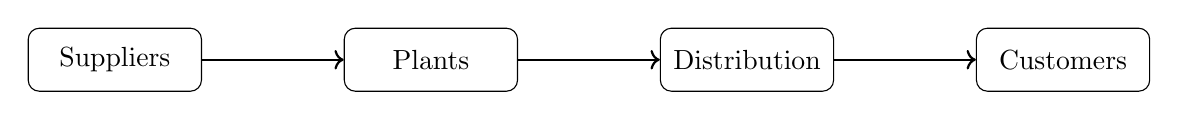
\begin{tikzpicture}[
    node distance=1.8cm,
    every node/.style={
        draw,
        rounded corners,
        minimum width=2.2cm,
        minimum height=0.8cm
    },
    arrow/.style={->, thick}
]

\node (s) {Suppliers};
\node (p) [right=of s] {Plants};
\node (d) [right=of p] {Distribution};
\node (c) [right=of d] {Customers};

\draw[arrow] (s) -- (p);
\draw[arrow] (p) -- (d);
\draw[arrow] (d) -- (c);

\end{tikzpicture}
\end{center}

\vspace{0.4cm}

The main challenges are:

\begin{itemize}
    \item Transportation costs
    \item Limited network capacity
    \item Efficient routing
    \item Vulnerability to disruptions
\end{itemize}

\end{frame}

% ------------------------------------------------
% Slide 3
% ------------------------------------------------
\begin{frame}{From Supply Chain to Graph}

We represent the supply chain as a graph:

\[
G=(V,E)
\]

\vspace{0.3cm}

\begin{columns}

\column{0.48\textwidth}

\textbf{Graph representation}

\begin{itemize}
    \item $V$: suppliers, plants, distribution centers, customers
    \item $E$: transportation routes
    \item $w_{ij}$: transportation cost
    \item $c_{ij}$: transportation capacity
\end{itemize}

\column{0.48\textwidth}

\begin{center}
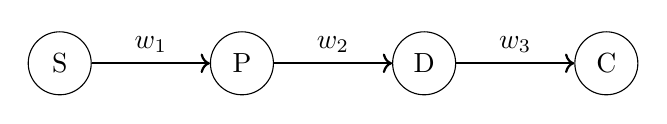
\begin{tikzpicture}[
    node distance=1.5cm,
    node/.style={
        circle,
        draw,
        minimum size=0.8cm
    },
    arrow/.style={->, thick}
]

\node[node] (a) {S};
\node[node] (b) [right=of a] {P};
\node[node] (c) [right=of b] {D};
\node[node] (d) [right=of c] {C};

\draw[arrow] (a) -- node[above] {$w_{1}$} (b);
\draw[arrow] (b) -- node[above] {$w_{2}$} (c);
\draw[arrow] (c) -- node[above] {$w_{3}$} (d);

\end{tikzpicture}
\end{center}

\end{columns}

\vspace{0.5cm}

\begin{center}
\textit{The graph transforms a complex supply chain into a mathematical network.}
\end{center}

\end{frame}

% ------------------------------------------------
% Slide 4
% ------------------------------------------------
\begin{frame}{Graph Theory Approach}

The analysis focuses on three questions:

\vspace{0.4cm}

\begin{enumerate}

    \item \textbf{Shortest Path}

    What is the most efficient route between two locations?

    \vspace{0.3cm}

    \[
    \min_{P}\sum_{(i,j)\in P} w_{ij}
    \]

    \item \textbf{Maximum Flow}

    How much product can move through the network?

    \vspace{0.3cm}

    \[
    \max \; \text{Flow}(s,t)
    \]

    \item \textbf{Network Resilience}

    What happens if a node or route fails?

\end{enumerate}

\vspace{0.4cm}

\begin{center}
\textbf{Python} is used to construct, visualize, and analyze the network.
\end{center}

\end{frame}

% ------------------------------------------------
% Slide 5
% ------------------------------------------------
\begin{frame}{The Supply Chain Network}

\begin{center}

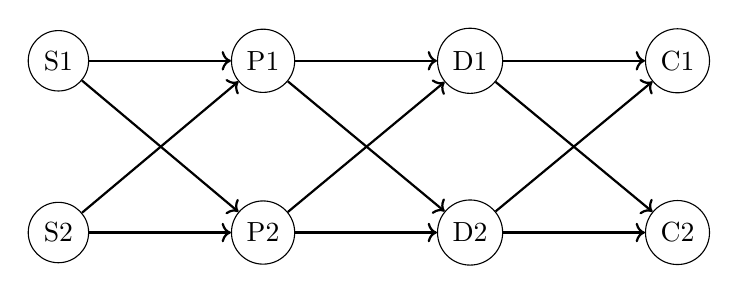
\begin{tikzpicture}[
    node distance=1.4cm and 1.8cm,
    every node/.style={
        circle,
        draw,
        minimum size=0.75cm
    },
    edge/.style={thick, ->}
]

\node (s1) {S1};
\node (s2) [below=of s1] {S2};

\node (p1) [right=of s1] {P1};
\node (p2) [right=of s2] {P2};

\node (d1) [right=of p1] {D1};
\node (d2) [right=of p2] {D2};

\node (c1) [right=of d1] {C1};
\node (c2) [right=of d2] {C2};

\draw[edge] (s1) -- (p1);
\draw[edge] (s1) -- (p2);
\draw[edge] (s2) -- (p1);
\draw[edge] (s2) -- (p2);

\draw[edge] (p1) -- (d1);
\draw[edge] (p1) -- (d2);
\draw[edge] (p2) -- (d1);
\draw[edge] (p2) -- (d2);

\draw[edge] (d1) -- (c1);
\draw[edge] (d1) -- (c2);
\draw[edge] (d2) -- (c1);
\draw[edge] (d2) -- (c2);

\end{tikzpicture}

\vspace{0.6cm}

\textbf{Network structure}

\begin{itemize}
    \item Multiple suppliers and production facilities
    \item Alternative transportation routes
    \item Different capacities and costs
    \item Potential bottlenecks
\end{itemize}

\end{center}

\end{frame}

% ------------------------------------------------
% Slide 6
% ------------------------------------------------
\begin{frame}{Scenario Analysis: Network Disruption}

\begin{columns}

\column{0.48\textwidth}

\textbf{Normal operation}

\begin{itemize}
    \item Maximum flow: $F_0$
    \item Transportation cost: $C_0$
    \item All facilities operational
\end{itemize}

\vspace{0.3cm}

\textbf{After disruption}

\begin{itemize}
    \item Remove a critical node or edge
    \item Recalculate maximum flow
    \item Identify new bottlenecks
\end{itemize}

\column{0.48\textwidth}

\begin{center}

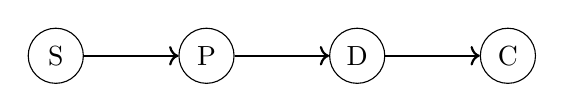
\begin{tikzpicture}[
    node distance=1.2cm,
    node/.style={
        circle,
        draw,
        minimum size=0.7cm
    },
    edge/.style={thick, ->}
]

\node[node] (a) {S};
\node[node] (b) [right=of a] {P};
\node[node] (c) [right=of b] {D};
\node[node] (d) [right=of c] {C};

\draw[edge] (a) -- (b);
\draw[edge] (b) -- (c);
\draw[edge] (c) -- (d);

\end{tikzpicture}

\vspace{0.4cm}

$\downarrow$

\vspace{0.4cm}

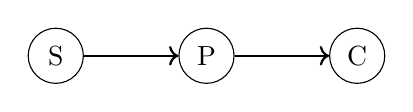
\begin{tikzpicture}[
    node distance=1.2cm,
    node/.style={
        circle,
        draw,
        minimum size=0.7cm
    },
    edge/.style={thick, ->}
]

\node[node] (a) {S};
\node[node] (b) [right=of a] {P};
\node[node] (d) [right=of b] {C};

\draw[edge] (a) -- (b);
\draw[edge] (b) -- (d);

\end{tikzpicture}

\end{center}

\end{columns}

\vspace{0.4cm}

\begin{center}
\textbf{Goal:} quantify the impact of disruptions on network performance.
\end{center}

\end{frame}

% ------------------------------------------------
% Slide 7
% ------------------------------------------------
\begin{frame}{Conclusions}

\begin{block}{Main Finding}
Graph theory provides a mathematical framework for analyzing complex supply chain networks.
\end{block}

\vspace{0.4cm}

\begin{itemize}

    \item \textbf{Shortest paths} identify efficient transportation routes.

    \item \textbf{Maximum flow} measures the capacity of the network.

    \item \textbf{Connectivity analysis} reveals critical infrastructure.

    \item \textbf{Scenario analysis} helps evaluate supply chain resilience.

\end{itemize}

\vspace{0.5cm}

\begin{center}
\Large
\textbf{Graph theory $\rightarrow$ Network structure $\rightarrow$ Economic decisions}
\end{center}

\end{frame}

\end{document}
